% !TEX root = epifanov_solid_state_physics.tex
%!TEX TS-program = pdflatex
%!TEX encoding = UTF-8 Unicode


\chapter[The Band Theory of Solids]{The Band Theory of Solids}\label{chap:5}
% \chaptermark{The Band Theory of Solids}

The theory of free electrons was the first successful attempt to explain the electric and magnetic properties of solids (primarily of metals). It was based on the assumption that metals contain free electrons capable of moving around the metal like gas molecules in a vessel. The theory of free electrons was successful in explaining such phenomena as the electric and the heat conductivities, thermionic emission, thermoelectric and galvanomagnetic effects, etc. However, this theory proved incapable of dealing with such properties of solids as are determined by their internal structure. It could not even explain why some bodies are conductors and some insulators.

The next stage in the progress of the electron theory has been the band theory of solids, which is outlined in this chapter.

\section{Electron energy levels of a free atom}\label{sec:37}

The state of an electron in an atom is determined by four quantum numbers: the principal $n$, the orbital $l$, the magnetic $m_l$, and the spin $\sigma$ numbers. In a hydrogen atom the \textit{principal quantum number}, $n$, describes the steady-state energy of the electron:
\begin{equation}\label{eq:5_1}
    E(n) = -\frac{R}{n^2}
\end{equation}

\noindent
where $R=\SI{13.6}{\electronvolt}$ is a universal constant, called a \textit{rydberg}---or the \textit{Rydberg constant}.

The \textit{orbital quantum number}, $l$, describes the orbital angular momentum of the electron, $\vec{p}_l$:
\begin{equation}\label{eq:5_2}
    p_l = \hslash \parenthesis{l (l + 1)}^{1/2}
\end{equation}

\noindent
($\hslash=h/2\pi$, with $h$ the Planck constant). The quantum number $l$ may assume only the following integral values:
\begin{equation*}
    l = 0, 1, 2, \ldots, (n - 1)
\end{equation*}

\noindent
$n$ value in all.

The \textit{magnetic quantum number}, $m_l$, describes the orientation of the orbital angular momentum with respect to some specified direction $\vec{H}$ [\fig{5_1}(a)]: the orientation of $\vec{p}_l$ with respect to $\vec{H}$ may only be such that its projection onto this direction is a multiple of $\hslash$:
\begin{equation}\label{eq:5_3}
    p_{lH} = m_l \hslash.
\end{equation}

\noindent
The number $m_l$ may assume the following set of integral values:
\begin{equation}\label{eq:5_3p}
    m_l = -l, -(l-1), \ldots, 0, 1, 2, \ldots, l. \tag{5.3$'$}
\end{equation}

\noindent
$21 + 1$ values in all.

\begin{figure}[t]
	\begin{center}
		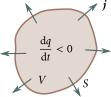
\includegraphics[scale=1]{figures/ch_05/fig_5_1.pdf}
		\caption[]{Orientations of orbital (a) and spin (b) angular momenta with respect to $\vec{H}$.}
		\label{fig:5_1}
	\end{center}
	\vspace{-0.7cm}
\end{figure}

Lastly, the \textit{spin quantum number}, $\sigma$, describes the orientation of the intrinsic angular momentum (the spin $\vec{p}_s$) of the electron with respect to specified direction $\vec{H}$ [\fig{5_1}(b)]: the vector $\vec{p}_s$ may only be oriented with respect to $\vec{H}$ so that its projection onto $\vec{H}$ is equal to
\begin{equation}\label{eq:5_4}
    p_{sH} = \sigma \hslash,
\end{equation}

\noindent
where only the values $+1/2$ and $-1/2$ being allowed for $\sigma$.

The states with orbital quantum number $l=0$ (the values of
other quantum numbers being irrelevant) are termed \textit{s states}; those with $l=1$, are termed \textit{p states}; with $l=2$, \textit{d states}; $l=0$, \textit{f states}; etc. Electrons in those states are termed s-, p-, d-, f-, etc. electrons.

In contrast to the hydrogen atom, the energy of an electron in many electron atoms depends not only on $n$ but on $l$ as well: $E=E(n,l)$. Only discrete values of $n$ and $l$ being allowed, the energy spectrum of electrons in atoms may assume only discrete values too; the spectrum consists of a set of allowed levels $E=E(n,l)$ separated by forbidden energy intervals. Table \ref{table:5_1} shows a diagram (not to scale) of the first three groups of such levels.

\begin{table}[!b]
	\renewcommand{\arraystretch}{1.2}
	\caption{}
	\vspace{-0.6cm}
	\label{table:5_1}
	\begin{center}\resizebox{0.98\linewidth}{!}{
			\begin{tabular}{lccc}
				\toprule[1pt]
				\textbf{Atomic energy} & & \textbf{Total number of} & \textbf{Splitting of levels into}\\
                \textbf{levels and} & $g=2l+1$ & \textbf{electrons on a} & \textbf{$g=2l+1$ sublevels}\\
                \textbf{their notation} & & \textbf{level: $n=2(2l+1)$} & \textbf{when degeneracy is lifted}\\
                \midrule[0.5pt]\midrule[0.5pt]
                & & & \multirow{3}{*}{\includegraphics[scale=0.8]{figures/ch_05/tab_5_1-1.pdf}}\\
                $E(3,2)$, \enlevel{2}{p} & $5$ & $10$ & \\
                & & &\\
                & & & \multirow{3}{*}{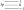
\includegraphics[scale=0.8]{figures/ch_05/tab_5_1-2.pdf}}\\
                $E(3,1)$, \enlevel{3}{p} & $3$ & $6$ & \\
                & & &\\
                $E(3,0)$, \enlevel{3}{s} & $1$ & $2$ & 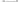
\includegraphics[scale=0.8]{figures/ch_05/tab_5_1-3.pdf}\\
                & & &
                \multirow{3}{*}{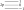
\includegraphics[scale=0.8]{figures/ch_05/tab_5_1-4.pdf}}\\
                $E(2,1)$, \enlevel{2}{p} & $3$ & $6$ &\\
                & & &\\
                $E(2,0)$, \enlevel{2}{s} & $1$ & $2$ &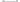
\includegraphics[scale=0.8]{figures/ch_05/tab_5_1-5.pdf}\\
                & & &\\
                $E(1,0)$, \enlevel{1}{s} & $1$ & $2$ &
                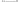
\includegraphics[scale=0.8]{figures/ch_05/tab_5_1-6.pdf}\\
                & & &\\
				\bottomrule[1pt]
			\end{tabular}
	}\end{center}
\end{table}

All the s levels are \textit{nondegenerate}. This means that everyone of them corresponds to a single electron state in the atom. In compliance with the Pauli exclusion principle there may be two electrons with opposite spins in such a state.

The p levels are three-fold degenerate: there is not one but three states with different magnetic quantum numbers $m_l$ to correspond to each of them. For $l=1$ those values are $m_l=-1, 0, +1$. Figure \ref{fig:5_2} shows the shape of electron clouds corresponding to those states. Since there may be two electrons per state, the total number of electrons in the p state is six.

\begin{figure}[t]
	\begin{center}
		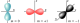
\includegraphics[scale=1]{figures/ch_05/fig_5_2.pdf}
		\caption[]{Electron clouds of the $2$p state.}
		\label{fig:5_2}
	\end{center}
	\vspace{-0.7cm}
\end{figure}

The degeneracy of the d levels is five-fold, since the allowed values of the magnetic quantum number for $l=2$ are $m_l=-2, -1, 0, +1, +2$. This level can accommodate $10$ electrons. Generally, a level with the orbital quantum number $l$ is a $(2l+1)$-fold degenerate one and can accommodate $2(2l+1)$ electrons.

When a free atom is placed in a strong external field, the degeneracy vanishes and every level splits into $(2l+1)$ closely spaced sublevels, as shown in the last column of \tab{5_1}.

The effect of an external field on different atomic levels is not the same. The splitting of the levels of inner electrons, whose interaction with the nucleus is strong, is so small that it may be neglected. As the shell radius is increased the energy of interaction of the respective electrons with the nucleus becomes smaller and the effect of the external field becomes more noticeable. The effect of an external field is most pronounced for the energy levels of outer electrons, whose bonds with the nucleus are relatively weak.

\section{Collectivization of electrons in a crystal}\label{sec:38}

The interatomic distances in solids are so small that every atom finds itself in a strong field of the neighbouring atoms. To gain insight into the effect this field exercises on the energy levels, consider
the following idealized example.

Arrange $N$ sodium atoms in the pattern of a three-dimensional lattice having the shape of a sodium crystal but with interatomic distances so great that the interaction between the atoms can be neglected. In this case, one can legitimately assume the energy states in every atom to be the same as in an individual sodium atom. Figure \ref{fig:5_3}(a) shows the energy diagram of two such atoms. Each of them has the appearance of a spindle-shaped potential trough inside of which the levels \enlevel{1}{s}{}, \enlevel{2}{s}{}, \enlevel{2}{p}{}, \enlevel{3}{s}{}, \ldots, are shown. The \enlevel{1}{s}{}, \enlevel{2}{s}{} and \enlevel{2}{p}{} levels in a sodium atom are fully occupied, the \enlevel{3}{s}{} is occupied to one half, and the levels above \enlevel{3}{s}{} are empty.

As shown in Figure \ref{fig:5_3}(a) the individual atoms are separated by potential barriers of the width $r\gg a$, where $a$ is the lattice constant. The height of the potential barrier $U$ is not the same for electrons occupying different levels. It is equal to the height measured from those levels to the zero level $00$. The potential barrier prevents the electrons from moving freely from one atom to another. Calculations show that for $r\approx\SI{30}{\angstrom}$ the average transition rate of a \enlevel{3}{s}{} electron from one atom to another is once in every \num{e20} years.

\begin{figure}[t]
	\begin{center}
		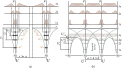
\includegraphics[scale=0.98]{figures/ch_05/fig_5_3.pdf}
		\caption[]{Variation of electronic states in approaching atoms: (a)---energy diagram of sodium atoms placed at a distance much greater than the sodium lattice parameter; (b)---energy diagram of sodium atoms brought together to a distance of the order of the lattice parameter.}
		\label{fig:5_3}
	\end{center}
	\vspace{-0.7cm}
\end{figure}

The upper part of Figure \ref{fig:5_3}(a) shows a qualitative picture of the space distribution of the density $\rho=4\pi\psi\psi^*$ of the probability of detecting electrons at a distance $r$ from the nucleus. The maxima of those curves correspond approximately to the radii of Bohr orbits of such electrons.

Now, make the lattice contract uniformly so that its symmetry remains unaffected. As the atoms are brought closer the interaction between them increases and for an interatomic distance equal to the lattice constant $a$ it turns into one characteristic of the crystal. Figure \ref{fig:5_3}(b) depicts that situation. We see that the walls of the potential troughs separating neighbouring atoms (they are shown in the figure by dotted lines) partly overlap to create new walls shown by solid lines that are lower than the zero level $00$.
Namely, the effect of the reduction of the interatomic distances is two-fold: to reduce the height and the width of the barrier, the latter to the value of the order of $a$. The height of the reduced barrier is $U_1'$ for \enlevel{1}{s}{}-, $U_2'$ for \enlevel{2}{s}{}-, and $U_3'$ for \enlevel{2}{p}{}-electrons, the original \enlevel{3}{s} levels of the sodium atoms lying above it. This fact makes it possible for the valence electrons of this level to move practically unhindered from one atom to another. The nature of the electron clouds of valence electrons shown in the upper part of the figure also points to the same conclusion: their overlapping is so complete that the density of the resulting cloud is practically uniform [\fig{5_3}(b)]. This corresponds to their complete collectivization in the lattice. Such collectivized electrons are usually termed \textit{free electrons} and the totality of them, the \textit{electron gas}.

A drastic reduction in the width and the height of the potential barrier brought about by the decrease in interatomic distances makes it possible for the electrons occupying other atomic levels, besides the valence levels, to move inside the crystal. Their motion takes place by means of tunneling through the barriers that separate neighbouring atoms. The narrower and the lower those barriers are, the more complete is the collectivization of the electrons and the greater is
their freedom.

\section{Energy spectrum of electrons in a crystal}\label{sec:39}

In the same way as the main goal of the theory of atoms is to describe the electron states in an atom and calculate the allowed energy levels, one of the main problems of the theory of the solid state is to determine the energy spectrum of the electrons in a crystal. One may obtain a qualitative idea about this spectrum using the following approximate method to treat the behaviour of electrons in a crystal.

To approximately describe the motion of an electron in a crystal we, may use the following Schr\"odinger equation:
\begin{equation}\label{eq:5_5}
    \nabla^2{\psi} + \frac{2m}{\hslash} (E-U) \psi = 0
\end{equation}

\noindent
where $U$ is the potential energy, $E$ the total energy, and $m$ the mass of the electron.

For electrons sufficiently strongly bound to the atoms the potential energy may be written in the form
\begin{equation}\label{eq:5_6}
    U = \ab{U}{a} + \delta{U}
\end{equation}

\noindent
where $\ab{U}{a}$ is the electron's energy in an isolated atom. In a crystal it is a periodic function with a period equal to the lattice parameter, since there is a recurrence in the value of energy as the electron moves from one atom to another (\fig{5_4}); $\delta{U}$ represents a correction that takes account of the effect of neighbouring atoms on this energy.

\begin{figure}[t]
	\begin{center}
		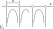
\includegraphics[scale=0.98]{figures/ch_05/fig_5_4.pdf}
		\caption[]{Periodic variation of electron potential energy in crystal.}
		\label{fig:5_4}
	\end{center}
	\vspace{-0.7cm}
\end{figure}

If one neglects the correction $\delta{U}$ in \eqn{5_6}, that is, considers only the zero approximation, one should take the wave function $\ab{\psi}{a}$ and the energy $\ab{E}{a}(n,l)$ of the electron in an isolated atom as the wave function and the energy of the electron in a crystal: $\psi=\ab{\psi}{a}, E=\ab{E}{a}(n,l)$, where $n$ and $l$ are the principal and orbital quantum numbers, which determine the energy of the electron in an atom.

In this case, the difference between a crystal and an isolated atom is that in an isolated atom a specified energy level $\ab{E}{a}(n,l)$ is unique, but in a crystal consisting of $N$ atoms there are $N$ such levels (\fig{5_5}). In other words, every energy level of an isolated atom is $N$-fold degenerate in a crystal. Such degeneracy is termed \textit{transpositional}.

\begin{figure}[t]
	\begin{center}
		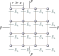
\includegraphics[scale=1]{figures/ch_05/fig_5_5.pdf}
		\caption[]{Each atomic energy level $\ab{E}{a}$ in a system consisting, of $N$ atoms is repeated $N$ times (is $N$-fold degenerate).}
		\label{fig:5_5}
	\end{center}
	\vspace{-0.7cm}
\end{figure}

Now let us estimate the correction $\delta{U}$ in the potential energy \eqref{eq:5_6}. As the isolated atoms are brought together to form a lattice, each atom increasingly feels the field of its neighbours with whom it interacts. As we have already seen, such interaction results in the lifting of degeneracy including transpositional degeneracy. Because of that, each level nondegenerate in an individual atom splits up into $N$ closely spaced sublevels to form an \textit{energy band}.

If every level in an isolated atom was $(2l+1)$ times degenerate, the corresponding band shall contain $N(2l+1)$ sublevels. Accordingly, the s level produces the s band consisting of $N$ sublevels and capable of carrying $2N$ electrons; the p level produces the p band consisting of $3N$ sublevels and capable of carrying $6N$ electrons; etc.

The separation between the sublevels in an energy band of an ordinary crystal is very small. A crystal of a volume of one cubic metre contains \num{e28} atoms. For a band of the order of \SI{1}{\electronvolt} wide, the separation between the sublevels is about \SI{e-28}{\electronvolt}. This separation is so negligible that the band may be considered to be practically continuous. However, the fact that the number of levels in a band is finite is very important for the determination of the distribution of electrons over states.

The maximum effect of the lattice field is on the external valence electrons. Because of that, the state of such electrons in a crystal experiences the greatest change and the energy bands formed by their energy levels are the widest. The internal electrons, which are strongly bound to their nuclei, are only slightly perturbed by the presence of neighbouring atoms and accordingly their energy bands in the crystal are almost as narrow as the levels of isolated atoms. Figure \ref{fig:5_6} shows a schematic diagram of energy band formation from discrete atomic levels.

\begin{figure}[t]
	\begin{center}
		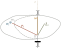
\includegraphics[scale=1]{figures/ch_05/fig_5_6.pdf}
		\caption[]{Schematic representation of energy band formation in a crystal from discrete atomic levels.}
		\label{fig:5_6}
	\end{center}
	\vspace{-0.7cm}
\end{figure}

Thus, in a crystal there is an \textit{allowed energy} band to correspond to each energy level of an isolated atom: the \enlevel{1}{s}{} band to correspond to the \enlevel{1}{s}{} level, the \enlevel{2}{p}{} band to the \enlevel{2}{p}{} level, etc. The allowed energy bands are separated by \textit{forbidden energy bands} $\ab{E}{g}$. As the energy of an electron in an atom is increased so is the width of the respective energy band, the width of the forbidden band being reduced.

Figure \ref{fig:5_7} shows the energy band structure of lithium, beryllium, and elements having the diamond lattice (diamond, silicon, germanium). In the lithium crystal [\fig{5_7}(a)], the splitting of the \enlevel{1}{s}{} level is a narrow one, the splitting of the \enlevel{2}{s}{} level being wider so that a sufficiently wide \enlevel{2}{s}{} energy band is formed. In the beryllium crystal [\fig{5_7}(b)], the \enlevel{2}{s}{} and the \enlevel{2}{p}{} bands overlap to form a mixed, or the so-called \textit{hybrid}, band. The situation is quite similar in case of the other elements of the main subgroup of Group II of the Mendeleev periodic table.

The pattern of band formation in crystals with the diamond lattice [\fig{5_7}(c)] is somewhat different. In this case, the bands formed from the s and the p levels overlap and split into two bands, so that each of them contains four states per atom: one s state and three p states. Those bands are separated by a forbidden band. The lower band is termed the \textit{valence band} and the upper the \textit{conduction band}.

\begin{figure}[t]
	\begin{center}
		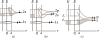
\includegraphics[scale=1.1]{figures/ch_05/fig_5_7.pdf}
		\caption[]{Formation of bands from atomic levels: (a)---in lithium crystal (band \enlevel{2}{s}{} is only half-filled); (b)---in beryllium crystal (filled \enlevel{2}{s}{} band and free \enlevel{2}{p}{} band overlap to form a partially filled hybrid band); (c)---in diamond-lattice elements of Group IV (the arrows denote the spin of the electrons).}
		\label{fig:5_7}
	\end{center}
	\vspace{-0.7cm}
\end{figure}

\section{Dependence of electron energy on the wave vector}\label{sec:40}

It was demonstrated in the preceding section that the pattern of the electron energy spectrum in a crystal is of a band type. Consider now the dependence of the electron energy $E$ on its momentum $p$ inside each band, that is, the shape of the $E(p)$ curves. The momentum dependence of $E$ is termed the \textit{dispersion law}, or \textit{dispersion relation}.

Turn now to the simplest case of a free electron moving along the $x$ axis and described by the following Schr\"odinger equation:
\begin{equation}\label{eq:5_7}
    \diffsec{\psi}{x} + \frac{2m}{\hslash} E \psi = 0
\end{equation}

\noindent
where
\begin{equation}\label{eq:5_8}
    E = \frac{p^2}{2m}
\end{equation}

\noindent
since a free electron has only kinetic energy.

Formula \eqref{eq:5_8} is the \textit{dispersion relation for free electrons}, which expresses the momentum dependence of $E$. It may be rewritten in the following form. According to the de Broglie formula
\begin{equation}\label{eq:5_9}
    p = \frac{h}{\lambda} = \frac{\hslash}{(\lambda/2\pi)} = \hslash k
\end{equation}

\noindent
where $\lambda$ is the wavelength of the electron, and
\begin{equation}\label{eq:5_10}
    k = \frac{2\pi}{\lambda}.
\end{equation}

\noindent
The vector $\vec{k}$ coinciding in direction with the direction of the electron wave propagation and equal in magnitude to $2\pi/\lambda$ is termed \textit{wave vector of the electron}. Substituting $p$ from \eqn{5_9} into \eqref{eq:5_8}, we obtain
\begin{equation}\label{eq:5_11}
    E = \frac{\hslash^2 k^2}{2m}.
\end{equation}

Equation \eqref{eq:5_11}, which expresses the dependence of the energy of a free electron on its wave vector, is just another form of writing the dispersion relation (the dispersion law) for such electrons.

It follows from Eqs. \eqref{eq:5_8} and \eqref{eq:5_11} that the dispersion law for free electrons is quadratic and for one-dimensional motion of the electron takes the form of a quadratic parabola shown in \fig{5_8}(a).

\begin{figure}[t]
	\begin{center}
		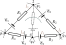
\includegraphics[scale=1.1]{figures/ch_05/fig_5_8.pdf}
		\caption[]{Motion of a free electron: (a)---dependence of energy on wave vector (dispersion curve); (b)---square modulus of wave function proportional to the probability of the electron being at point $x$.}
		\label{fig:5_8}
	\end{center}
	\vspace{-0.7cm}
\end{figure}

The solution of \eqn{5_7} is a travelling plane wave
\begin{equation}\label{eq:5_12}
    \psi = C e^{ikx}
\end{equation}

\noindent
where $C$ is the wave's amplitude.

As is well known, the square of the modulus of the wave function is proportional to the probability of detecting the electron in a specified region of space. As may be seen from \eqn{5_12}, for a free electron this probability is independent of the electron's position since
\begin{equation}\label{eq:5_13}
    \absolute{\psi}^2 = \psi\psi^* = C^2
\end{equation}

\noindent
which means that for a free electron every point in space is equivalent and the probability of detecting it is everywhere the same (\fig{5_8}(b)).

The case of an electron moving in a periodic field of a crystal formed by regularly arranged ions is different (\fig{5_9}). The probability of detecting it in a specified point of the crystal should be a periodic function in $x$, since positions displaced from one another by a multiple of the lattice constant $a$ (for instance, the positions D, D$'$ and B in \fig{5_9}) are equiprobable for the electron. The positions inside a period $a$ (for example, inside DFD$'$) are, however, all different. This means that the amplitude of the wave function $\psi(x)$ of an electron moving in a periodic field does not, as in the case of a free electron, stay constant but changes periodically, or it may be said to be modulated with a period equal to the lattice parameter $a$. Denote this amplitude $u(x)$. Then, the wave function of the electron moving in a periodic field of a crystal in the direction of the $x$
axis may be expressed in the following form:
\begin{equation}\label{eq:5_14}
    \psi(x) = u(x) e^{ikx}
\end{equation}

\noindent
where $u(x+na)=u(x)$, where $n$ is an arbitrary integer. Relation \eqref{eq:5_14} is termed the \textit{Bloch function}. The specific form of this function is determined by the potential energy $U(x)$, which enters into the Schr\"odinger equation \eqref{eq:5_5}.

\begin{figure}[t]
	\begin{center}
		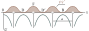
\includegraphics[scale=1]{figures/ch_05/fig_5_9.pdf}
		\caption[]{Motion of an electron in periodic field. The square modulus of the wave function that describes the probability of the electron being at point $x$ of the horizontal axis is a periodic function of coordinate $x$, the period being equal to the lattice parameter $a$.}
		\label{fig:5_9}
	\end{center}
	\vspace{-0.7cm}
\end{figure}

There should be a corresponding change in the dispersion relation for electrons moving inside a crystal as compared with that for free electrons. Firstly, as we have already seen, the energy spectrum of such electrons assumes a band pattern: allowed energy bands formed from corresponding atomic levels $\ab{E}{a}$ are separated by forbidden energy bands. Secondly, calculations show the electron energy inside each hand to be a function of the wave vector $k$, which for a one-dimensional crystal (an atomic chain) with the parameter $a$ is of the form
\begin{equation}\label{eq:5_15}
    E(k) = \ab{E}{a} + C + 2 A \cos(ka)
\end{equation}

\noindent
where $\ab{E}{a}$ is the energy of the atomic level from which the band was formed; $C$ is the displacement of this level due to the effect of the field of neighbouring atoms; $A$ is the so-called \textit{exchange integral}, which takes into account the newly created probability for an electron to move from one atom to another owing to the overlapping of the atomic wave functions [\fig{5_3}(b)]. The exchange integral is the greater the greater the overlapping of the wave functions, that is, the greater is the exchange rate of the electrons of neighbouring atoms. For s states $\ab{A}{s}<0$, for p states $\ab{A}{p}>0$, therefore, it is reasonable to write out relation \eqref{eq:5_15} individually for the s and the p bands. For the s bands
\begin{equation}\label{eq:5_16}
    \ab{E}{s}(k) = \ab{E}{s}' - 2 \ab{A}{s} \cos(ka)
\end{equation}

\noindent
and for the p bands
\begin{equation}\label{eq:5_17}
    \ab{E}{p}(k) = \ab{E}{p}' - 2 \ab{A}{p} \cos(ka)
\end{equation}

\noindent
where $\ab{E}{s}'=\ab{E}{as}+\ab{C}{s}$, $\ab{E}{p}'=\ab{E}{ap}+\ab{C}{p}$, and $\ab{A}{s}$ and $\ab{A}{p}$ are the absolute values of the exchange integrals for the respective states.

Figure \ref{fig:5_10} shows dispersion curves $E(k)$ for the s and p bands drawn to satisfy equations \eqref{eq:5_16} and \eqref{eq:5_17}. For the s states, $\ab{E}{s}$ at $k=0$ assumes its minimum value $\ab{E}{s,min}=\ab{E}{s}'-2\ab{A}{s}$.
As $k$ increases, $\cos(ka)$ decreases and the value of $\ab{E}{s}(k)$ rises reaching its maximum $\ab{E}{s,max}=\ab{E}{s}'+2\ab{A}{s}$ at $k=\pi/a$. In the interval of values of $k$ from $0$ to $-\pi/a$, $\ab{E}{s}(k)$ changes in a similar fashion.
The width of the allowed s band from $\ab{E}{s,min}$ to $\ab{E}{s,max}$ is
\begin{equation}\label{eq:5_18}
    \Delta{\ab{E}{s}} = \ab{E}{s,max} - \ab{E}{s,min} = 4 \ab{A}{s}.
\end{equation}

\noindent
As may be seen, it is determined by the absolute value of the exchange integral, which, in its turn, depends on the overlapping of wave functions of neighbouring atoms. The shape of the curve $\ab{E}{s}(k)$ is that of
an overturned bell.

\begin{figure}[t]
	\begin{center}
		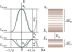
\includegraphics[scale=1]{figures/ch_05/fig_5_10.pdf}
		\caption[]{Dispersion curves for an electron moving in a periodic field: the lower curve corresponds to the s band, the upper curve to the p band; dotted lines are parabolas expressing the $E(k)$ dependence in the centre and on the boundaries of the Brillouin zone.}
		\label{fig:5_10}
	\end{center}
	\vspace{-0.7cm}
\end{figure}

For the p states $\ab{E}{p,min}=\ab{E}{p}'-2\ab{A}{p}$ corresponds to $k=\pm\pi/a$, and at $k=0$, $\ab{E}{p,max}=\ab{E}{p}'+2\ab{A}{p}$. The width of the p band
\begin{equation}\label{eq:5_19}
    \Delta{\ab{E}{p}} = \ab{E}{p,max} - \ab{E}{p,min} = 4 \ab{A}{p}
\end{equation}

\noindent
as in the previous case, is determined by the absolute value of the exchange integral $\ab{A}{p}$. As a rule, the higher the atomic level the greater the overlapping of the corresponding wave functions in the crystal, the greater the value of the exchange integral, and the wider the energy band formed from this level. For this reason, high atomic levels are the origin of wide energy bands separated by narrow forbidden bands (see \fig{5_6}).

The intervals of $k$ inside which the electron energy $E(k)$ as a periodic function of $k$ completes its full cycle are termed \textit{Brillouin zones}. For a one-dimensional crystal (an atomic chain) the first Brillouin zone lies between $k=-\pi/a$ and $k=\pi/a$ and is $2\pi/a$ wide (\fig{5_10}). In the vicinity of a dispersion curve's extremum, that is, in the vicinity of $k=0$ and $k=\pm\pi/a$ (the centre and the boundary of the first Brillouin zone), $\cos(ka)$ can be expanded into a power series in $ka$ ($k$ is measured from $0$ if the extremum is in the centre of the Brillouin zone and from $\pm\pi/a$ if it is on its boundary) leaving only two terms of the expansion
\begin{equation*}
    \cos(ka) = 1 - \frac{(ka)^2}{2} + \ldots.
\end{equation*}

\noindent
Substituting this into Eqs. \eqref{eq:5_16} and \eqref{eq:5_17}, we obtain $\ab{E}{s}(k)=\ab{E}{s,min}+\ab{A}{s}(ka)^2$ and $\ab{E}{p}(k)=\ab{E}{p,max}-\ab{A}{p}(ka)^2$.
The minimum of the dispersion curve $E(k)$ is termed the \textit{bottom of the energy band} and the maximum the \textit{top of the band}. Therefore, we may rewrite the sought for relations in a more general form:
\begin{equation}\label{eq:5_20}
    \ab{E}{bottom}(k) = \ab{E}{min} + A (ka)^2
\end{equation}

\noindent
for the bottom of the band, and
\begin{equation}\label{eq:5_21}
    \ab{E}{top}(k) = \ab{E}{max} - A' (ka)^2
\end{equation}

\noindent
for the top of the band.

Hence, close to the top and the bottom of an energy band the portion of the electron energy that depends on the wave vector is proportional to the square of the wave vector, measured in the way indicated above, and to the exchange integral that determines the width of the band. The parabolas corresponding to equations \eqref{eq:5_20} and \eqref{eq:5_21} are shown in \fig{5_10} by dotted lines.

The $E(k)$ dependence for real crystals is, as a rule, much more complex than that expressed by \eqn{5_15}.

Figure \ref{fig:5_11}(a) shows the dispersion curves for the bottom of the conduction band (curve $1$) and the top of the valence band (curve $2$) of silicon. We see that the bottom of the conduction band, D, of silicon is not in the centre of the Brillouin zone but near its boundary in the direction $[100]$. The valence band is bounded by a curve in the shape of a parabola with its apex at B in the centre of the Brillouin zone. However, despite such complexity of the dispersion curves, the quadratic dependence of $E(k)$ expressed by formulae \eqref{eq:5_20} and \eqref{eq:5_21} remains valid for both band-edges in this case.

\begin{figure}[t]
	\begin{center}
		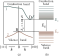
\includegraphics[scale=1]{figures/ch_05/fig_5_11.pdf}
		\caption[]{Band pattern of silicon: (a)---dispersion curves $E(k)$ bounding the conduction band (curve $1$) and the valence band (curve $2$); the energy minimum of the conduction band is at point D in the $[100]$ direction, energy maximum of the valence band is in the Brillouin zone centre B; the distance between minimum D and maximum B is the forbidden band width $\ab{E}{g}$; (b)---schematic representation of energy band pattern of silicon.}
		\label{fig:5_11}
	\end{center}
	\vspace{-0.7cm}
\end{figure}

The width of the forbidden band, or \textit{energy gap}, is determined by the minimum gap between the valence and the conduction bands; in \fig{5_11}(a) this is denoted by $\ab{E}{g}$.

Frequently, when making a simplified analysis of the energy-band structure of semiconductors, instead of the actual dispersion curves, which bound the valence and the conduction band, use is made of two parallel lines, one drawn tangentially to the bottom of the conduction band and the other to the top of the valence band [\fig{5_11}(b)]. The first line is taken to represent the lower boundary (the bottom) of the conduction band and the second the upper boundary (the top) of the valence band. The separation between the lines is equal to the forbidden band width $\ab{E}{g}$.

\section{Effective mass of the electron}\label{sec:41}

The de Broglie formula establishes the following relation between the momentum of a free electron and its wave vector:
\begin{equation*}
    \vec{p} = \hslash \vec{k}.
\end{equation*}

\noindent
The velocity of the electron's translational motion is
\begin{equation}\label{eq:5_22}
    \vec{v} = \frac{\vec{p}}{m} = \parenthesis{\frac{\hslash}{m}} \vec{k}.
\end{equation}

\noindent
Differentiating \eqref{eq:5_11} with respect to $k$, we obtain
\begin{equation*}
    k = \frac{m}{\hslash^2} \diff{E}{k}.
\end{equation*}

\noindent
Substituting this into \eqref{eq:5_9} and \eqref{eq:5_22} we obtain
\begin{equation}\label{eq:5_23}
    p = \hslash k = \frac{m}{\hslash} \diff{E}{k},\quad v = \frac{\hslash}{m} k = \frac{1}{\hslash} \diff{E}{k}.
\end{equation}

Expressions for the momentum and for the velocity of translational motion written in this form turn out to be valid not only for free electrons but for electrons moving in a periodic crystal field as well. Momentum $\vec{p}$ is in the latter case termed \textit{quasimomentum} of the electron.

Set up an external field $\pmb{\mathscr{E}}$ in the crystal. This field acts on the electron with a force
\begin{equation*}
    \vec{F} = - q \pmb{\mathscr{E}}
\end{equation*}

\noindent
imparting to it an acceleration
\begin{equation*}
    j = \diff{v}{t} = \frac{1}{\hslash} \diff{}{t}\parenthesis{\diff{E}{k}} = \frac{1}{\hslash} \diffn{E}{k}{2} \diff{k}{t}.
\end{equation*}

\noindent
The work performed by the force $F$ during the interval $\deriv{t}$ is
\begin{equation*}
    \deriv{W} = F \vec{v}\, \deriv{t} = \frac{F}{\hslash} \diff{E}{k}\, \deriv{t}.
\end{equation*}

\noindent
This work is spent on increasing the electron's energy by an amount $\deriv{E}$, where $\deriv{E}=(F/\hslash) (\diffin{E}{k})\,\deriv{t}$. Hence, $F/\hslash= \diffin{k}{t}$. Substituting into the right-hand side of the expression for $j$, we obtain
\begin{equation}\label{eq:5_24}
    j = \frac{F}{\hslash^2} \diffn{E}{k}{2} = -\frac{q\mathscr{E}}{\hslash^2} \diffn{E}{k}{2} = -\frac{q\mathscr{E}}{\ab{m}{eff}}.
\end{equation}

Equation \eqref{eq:5_24} establishes the relation between the electron's acceleration $j$ and the external force $F$ with which an external field $\pmb{\mathscr{E}}$ acts on it. Hence, it is an expression of Newton's second law. It follows then that the electron acted upon by an external force moves in a periodic crystal field on the average in the same way as a free electron would move if its mass were
\begin{equation}\label{eq:5_25}
    \ab{m}{eff} = \hslash^2 \parenthesis{\diffn{E}{k}{2}}^{-1}.
\end{equation}

\noindent
The mass $\ab{m}{eff}$ is called the \textit{effective mass of the electron}. Having attributed to the electron in a periodic crystal field a mass $\ab{m}{eff}$, we may now regard it as being free and describe its motion in an external field in the same way as we would describe the motion of an ordinary free electron.

However, the effective mass, which embraces all the details of electron motion in a periodic crystal field, is a very particular quantity. To begin with, it may be positive or negative, many times larger or many times smaller in magnitude than the electron's rest mass $m$. Let us make a more detailed study of the problem.

For electrons close to the bottom of a band the energy is $\ab{E}{bottom}=\ab{E}{min}+A(ka)^2$, the second derivative with respect to $k$ being $\diffnin{E}{k}{2}=2Aa^2$. Substituting into \eqn{5_25}, we obtain the following expression for the effective mass of the electron, which we shall denote
$\ab{m}{n}$:
\begin{equation}\label{eq:5_26}
    \ab{m}{n} = \frac{\hslash^2}{2 A a^2}.
\end{equation}

\noindent
Since $A>0$, we see that $\ab{m}{n}>0$. Hence, electrons close to the bottom of an energy band have a positive effective mass. For this reason, they behave normally in an external field, accelerating in the direction of the acting force. The difference between such electrons and free electrons is that their mass may be quite different from the rest mass. It may be seen from \eqn{5_26} that the greater $A$ is, that is, the wider the allowed band, the less the effective mass of the electrons occupying states close to the bottom of the band is.

For electrons close to the top of the band the energy is $\ab{E}{top}=\ab{E}{max}-A'(ka)^2$, the second derivative of $E$ with respect to $k$ being $\diffnin{E}{k}{2}=-2A'a^2$, and the effective mass, which we denote $\ab{m}{n}'$, is
\begin{equation}\label{eq:5_27}
    \ab{m}{n}' = - \frac{\hslash^2}{2 A' a^2}.
\end{equation}

\noindent
It is a negative quantity. Such electrons behave abnormally in an external field set up in a crystal: they are accelerated in the direction opposite to the acting force. The absolute value is, as before, determined by the width of the energy band: $\ab{m}{n}'$ is the smaller the wider the band is.

Let us now find what is responsible for such a ``strange'' behaviour of the electron in a crystal.

In case of a free electron, all the work $W$ performed by an external force $\vec{F}$ is spent to increase the kinetic energy of the electron's translational motion:
\begin{equation*}
    W = \ab{E}{k} = \frac{mv^2}{2} = \frac{\hslash^2 k^2}{2m}.
\end{equation*}

\noindent
Differentiating $\ab{E}{k}$ twice with respect to $k$, we obtain, $\diffnin{E_k}{k}{2}=\hslash^2/m$. Substituting into \eqn{5_25}, we find that $\ab{m}{eff}=m$. Hence, the effective mass of a free electron is simply its rest mass.

The situation may be quite different in a crystal where the electron has not only kinetic energy but potential energy as well. When the electron moves under the action of an external force $\vec{F}$, some of the work performed by this force may be transformed into kinetic energy $\ab{E}{k}'$, the rest being transformed into potential energy $U$, and $W=\ab{E}{k}'+U$. In this case, the result will be a smaller increase in kinetic energy and, consequently, in electron velocity than in the case of a free electron. The electron, figuratively speaking, gains weight and moves under the action of the force $\vec{F}$ with a smaller acceleration than a free electron would.

Should the entire work of the external force be transformed into potential energy $U$, that is $W=U$, there would be no increase in the kinetic energy and in the velocity of the electron and it would behave as a particle of infinite effective mass.

Finally, if in the course of the electron's motion, not only the entire work of the external force $\vec{F}$, but some of the kinetic energy $\ab{E}{k}'$ that the electron had initially, too shall be transformed into the potential energy, so that $U=W+\ab{E}{k}'$, then as the electron moves along the crystal its velocity shall diminish, it shall be accelerated, behaving as a particle with a \textit{negative effective mass}. Just such is the behaviour of electrons occupying states close to the top of the conduction band.

However, a situation is possible in a crystal when in the course of the electron's motion under the action of an external force $\vec{F}$, not only the entire work of this force but some of the electron's potential
energy, say $U'$, shall be transformed into its kinetic energy, so that $\ab{E}{k}''=W+U'$, The $\ab{E}{k}''$ and the velocity $v$ of such an electron shall rise quicker than those of a free electron. It looses weight as compared with the free electron, so that its effective mass $\ab{m}{eff}<m$.

The aforesaid is illustrated in \fig{5_12}, which shows the nature of the variation of the total energy of the electron $E(k)$, of its translational velocity $v(k)$, and of its effective mass $\ab{m}{eff}$ with the rise in $k$ from $0$ to $\pm\pi/a$.

\begin{figure}[t]
	\begin{center}
		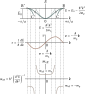
\includegraphics[scale=1]{figures/ch_05/fig_5_12.pdf}
		\caption[]{Dependence of electron energy $E$, group velocity $v$, and effective electron mass $\ab{m}{eff}$ on $k$.}
		\label{fig:5_12}
	\end{center}
	\vspace{-0.7cm}
\end{figure}

Close to the bottom of the band ($k=0$), as long as the electron's energy $E(k)$ rises approximately in proportion to $k^2$, the velocity of the electron's translational motion $v\propto\diffin{E}{k}$ increases in proportion to $\ab{m}{n}$, the acceleration remains positive, and the effective mass $\ab{m}{eff}\propto\parenthesis{\diffnin{E}{k}{2}}^{-1}$ retains its constant positive value $\ab{m}{n}$.
At the point of inflection C of the curve $E(k)$, the second derivative $\diffnin{E}{k}{2}$ vanishes and the first derivative reaches its maximum value. Therefore,
as this point is approached, $\ab{m}{eff}\to\infty$ and $v\to\ab{v}{max}$. After the point of inflection, $\diffin{E}{k}$ starts to decrease causing a decrease in $v$; hence, acceleration becomes negative, which, for the direction of the external force $\vec{F}$ remaining unchanged, is equivalent to a change in the sign of the effective mass from the positive to the negative. If the curvature of the curve $E(k)$, which is proportional to $\diffnin{E}{k}{2}$, also changes, this would lead to a change in the absolute value of $\ab{m}{eff}\propto\parenthesis{\diffnin{E}{k}{2}}^{-1}$.
Near the top of the band $E(k)$ again becomes a quadratic function of $k$, and the effective mass assumes a constant negative value $\ab{m}{n}'$.

\section[Occupation of bands by electrons]{Occupation of bands by electrons. Conductors, dielectrics, and semiconductors}\label{sec:42}

Each energy band contains a limited number of energy levels. In compliance with the Pauli exclusion principle each level may be occupied by no more than two electrons. With the limited number of electrons in a solid only the lower energy bands will be filled.
According to the nature of band occupation by electrons all solids can be classified into two large groups.

The \textit{first} group includes bodies in which there is a partially filled band above the completely filled lower bands [\fig{5_13}(a)]. Such bands are formed from partially filled atomic levels as, for instance, in the case of alkali metals. A partially filled band may also be the result of overlapping of filled and empty or partially filled bands, as is the case with beryllium and alkali-earth metals [\fig{5_13}(b)]. A partially filled band is a feature of metals.

\begin{figure}[t]
	\begin{center}
		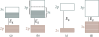
\includegraphics[scale=1]{figures/ch_05/fig_5_13.pdf}
		\caption[]{Occupation of bands by electrons: (a, b)---there is a partially filled band above the filled band; (c, d)---there is an empty band above the filled band.}
		\label{fig:5_13}
	\end{center}
	\vspace{-0.7cm}
\end{figure}

The \textit{second} group includes bodies with empty bands above completely filled ones [\fig{5_13}(c,d)]. Typical examples of such bodies are the elements of Group IV of the Mendeleev periodic table---carbon in the diamond modification, silicon, germanium and gray tin, which has the structure of diamond. This group also includes many chemical compounds---metal oxides, nitrides, carbides, halides of alkali metals, etc.

According to the band theory of solids, the electrons of the outermost energy bands have practically the same freedom of movement, no matter whether the solid is a metal or a dielectric. The motion takes place by means of tunneling from atom to atom. Despite this fact, there is a difference of many orders of magnitude in the electric properties, in particular in the electrical conductivity, of the bodies of both types: in metals $\sigma\approx\num{e7}(\si{\ohm\metre})^{-1}$, and in good dielectrics $\sigma\approx\num{e-11}(\si{\ohm\metre})^{-1}$.

To gain insight into the mechanism of electrical conductivity of solids let us discuss the behaviour of the electrons of partially and completely filled energy bands in an external field.

Set up an external field $\pmb{\mathscr{E}}$ in the crystal. This field acts on every electron with a force $\vec{F}=-q\pmb{\mathscr{E}}$ that tends to distort the symmetry in the velocity distribution of the electrons, so that those moving against the force are decelerated and those moving in the direction of the force are accelerated. Since such acceleration and deceleration
inevitably entail a change in the electron's energy, this is equivalent to the electron's transition to states with higher or lower energies. Such transitions may, evidently, take place only if there are unoccupied states inside the band to which the electrons belong, that is, if the band is not completely filled. In this case, even a weak electric field is capable of imparting to the electrons the necessary additional momentum that will take them to nearby free levels. A prevailing motion of the electrons in the direction opposite to that of the field will be set up in the solid resulting in an electric current. Such solids should be good conductors, which is actually the case.

Now let us imagine that the valence band of the crystal is completely filled and is separated from the nearby empty band by a wide energy gap $\ab{E}{g}$ [\fig{5_13}(c)]. An external field applied to such a crystal is incapable of changing the nature of electron motion in the valence band because it is unable to lift the electrons to the empty band lying above it. Inside the valence band, which has no free levels, the field may only cause the electrons to change places and this
does not distort the symmetry of the electron distribution over velocities. Therefore, in such solids an external field is incapable of inducing directional motion of the electrons, that is, an electric current, and the electrical conductivity of such solids should be practically zero.

Hence, for a body to have high electrical conductivity it must have in its energy spectrum some energy bands only partially filled with electrons, as is the case with the typical metals [\fig{5_13}(a,b)]. The absence of such bands in solids belonging to the second group makes them \textit{nonconductors} despite the fact that they contain electrons weakly bonded to individual atoms.

The solids of the second group are conventionally subdivided into dielectrics and semiconductors according to the width of the forbidden band. \textit{Dielectrics} include solids with a relatively wide forbidden band. For typical dielectrics, $\ab{E}{g}>\SI{3}{\electronvolt}$. For diamond, $\ab{E}{g}=\SI{5.2}{\electronvolt}$; for boron nitride, $\ab{E}{g}=\SI{4.6}{\electronvolt}$; for $\ce{Al2O3}$, $\ab{E}{g}=\SI{7}{\electronvolt}$; etc.

\textit{Semiconductors} include solids with a relatively narrow forbidden band [\fig{5_13}(d)]. For typical semiconductors, $\ab{E}{g}\lesssim\SI{1}{\electronvolt}$. Thus, for germanium, $\ab{E}{g}=\SI{0.66}{\electronvolt}$; for silicon, $\ab{E}{g}=\SI{1.08}{\electronvolt}$; for indium antimonide, $\ab{E}{g}=\SI{0.17}{\electronvolt}$; for gallium arsenide, $\ab{E}{g}=\SI{1.43}{\electronvolt}$; etc.

Let us consider this class of solids in more detail.

\section{Intrinsic semiconductors. The concept of a hole}\label{sec:43}

\textbf{Intrinsic semiconductors.} Semiconductors containing a negligible amount of electro-active defects (chemical and crystallographic) are termed \textit{intrinsic semiconductors}. They include some pure chemical elements (germanium, silicon, selenium, tellurium, etc.) and numerous chemical compounds such as gallium arsenide (\ce{GaAs}), indium arsenide (\ce{InAs}), indium antimonide (\ce{InSb}), silicon carbide (\ce{SiC}), etc.

Figure \ref{fig:5_14}(a) shows a simplified schematic diagram of an intrinsic semiconductor. At absolute zero, its valence band is completely filled and the conduction band, which is a distance $\ab{E}{g}$ above the valence band, is empty. For this reason, at absolute zero, the intrinsic semiconductor, same as a dielectric, has zero conductivity.

\begin{figure}[t]
	\begin{center}
		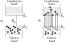
\includegraphics[scale=1]{figures/ch_05/fig_5_14.pdf}
		\caption[]{Intrinsic semiconductor: (a)---at absolute zero the valence band is completely filled by electrons and the conduction band is completely empty; (b)---at temperatures above absolute zero part of the electrons from the valence band are excited to the conduction band; holes appear in the valence band and free electrons in the conduction band (white circles denote holes and black circles denote electrons); $\ab{E}{c}$ is the bottom of conduction band and $\ab{E}{v}$ is the top of valence band.}
		\label{fig:5_14}
	\end{center}
	\vspace{-0.7cm}
\end{figure}

However, as the temperature increases the electrons of the valence band become excited and some of them receive enough energy to surmount the forbidden band and go over to the conduction band [\fig{5_14}(b)]. This results in free conduction electrons appearing in
the conduction band and in free electron levels capable of accepting valence band electrons appearing in the valence band. When an external field is applied to such a crystal, a directional motion of the electrons of the conduction and the valence bands is established, resulting in the appearance of an electric current. The crystal becomes conducting.

The narrower the forbidden band and the higher the crystal's temperature the greater the number of electrons going over to the conduction band and, correspondingly, the greater the crystal's electrical conductivity. For instance, for germanium with $\ab{E}{g}=\SI{0.66}{\electronvolt}$, the concentration of the electron gas in the conduction band already at room temperature is as high as $\ab{n}{i}\approx\SI{e19}{\per\metre\cubed}$ and specific resistance is as low as $\ab{\rho}{i}\approx\num{0.48}(\si{\ohm\metre})^{-1}$.
At the same time, for diamond with $\ab{E}{g}=\SI{5.2}{\electronvolt}$, $\ab{n}{i}$ at room temperature is only about \SI{e4}{\per\metre\cubed} and $\ab{\rho}{i}\approx\num{e8}(\si{\ohm\metre})^{-1}$. However, already at $T=\SI{600}{\kelvin}$, the electron gas concentration in diamond increases by many orders of magnitude and its specific resistance becomes as low as that of germanium at room temperature.

Two important conclusions may be drawn from the above.
\begin{enumerate}[(1)]
    \item The electrical conductivity of an intrinsic semiconductor is an excited conductivity: it appears only as a result of the action of some external factor capable of imparting sufficient energy to the electrons of the valence band to move them over to the conduction
    band. Such factors may be heating of the semiconductor and irradiation with light or with ionizing radiation.

    \item The division of materials into semiconductors and dielectrics is essentially a matter of convention. Diamond---a dielectric at room     temperature---exhibits a noticeable conductivity at higher temperatures and may also be considered to be a semiconductor. Materials with ever increasing forbidden band widths are now being used as semiconductors, gradually making the division into semiconductors and dielectrics irrelevant.
\end{enumerate}

\textbf{The concept of a hole.} Let us now discuss in more detail the behaviour of the electrons in the valence band in which as a result of transition of some of the electrons to the conduction band some free levels have appeared [\fig{5_14}(b)].

Now, the electrons of the valence band acted upon by an external field can go over to the free levels and establish an electric current in the crystal. Let us find the instantaneous value of this current.

The current established by one electron moving with a velocity $\vec{v}_i$ is
\begin{equation*}
    \vec{I}_i = -q \vec{v}_i.
\end{equation*}

\noindent
The total instantaneous current established by all the electrons of the valence band is
\begin{equation*}
    \ab{\vec{I}}{t} = -q \sum_i \vec{v}_i.
\end{equation*}

\noindent
where the sum is over all the states occupied by electrons.

For a band completely filled with electrons, $\ab{\vec{I}}{t}=0$, since there is an electron with the velocity $\vec{v}_i$ to correspond to every electron with the velocity $-\vec{v}_i$.

Now let us imagine that all the states in the valence band except one with the velocity $\vec{v}_s$ are filled. The total current in such a band will be
\begin{equation*}
    \vec{I} = -q \sum_{i\neq s}\vec{v}_i = -q \sum_i \vec{v}_i + q \vec{v}_s.
\end{equation*}

\noindent
Since the first term in the right-hand side is zero,
\begin{equation}\label{eq:5_28}
    \vec{I} = q \vec{v}_s.
\end{equation}

Hence, the total current of all the electrons in a valence band with one vacant state is equivalent to a current set up by the motion of one particle with a positive charge $q$ occupying the respective state. Such a fictitious particle is called a \textit{hole}. If we attribute to the hole a positive charge $+q$ numerically equal to the electron charge, we should also attribute to it a positive effective mass $\ab{m}{p}$ numerically equal to the negative effective mass of the electron $\ab{m}{n}'$, which initially occupied that state close to the top of the valence band, since only in this case will the current established by holes coincide both in magnitude and in direction with the current established by the electrons of the almost completely filled valence band.

Table \ref{table:5_2} presents the room temperature electrophysical properties and characteristics of the band pattern of three typical intrinsic semiconductors---silicon, germanium, and indium antimonide.

\begin{table}[!b]
	\renewcommand{\arraystretch}{1.2}
	\caption{}
	\vspace{-0.6cm}
	\label{table:5_2}
	\begin{center}\resizebox{0.98\linewidth}{!}{
			\begin{tabular}{lccccc}
				\toprule[1pt]
                \multirow{2}{*}{\textbf{Semiconductor}} & \multirow{2}{*}{$\ab{E}{g}, (\si{\electronvolt})$} & \multirow{2}{*}{$\ab{n}{i}, \parenthesis{\si{\per\metre\cubed}}$} & \multirow{2}{*}{$\ab{\rho}{i}, (\si{\ohm\metre})$} & \multicolumn{2}{c}{\textbf{Effective mass}}\\
                \cline{5-6}
                & & & & $\ab{m}{n}$ & $\ab{m}{p}$\\
                \midrule[0.5pt]\midrule[0.5pt]
                Silicon & $1.12$ & $\sim\num{e16}$ & \num{2e3} & $1.08 m$ & $0.37 m$\\
                Germanium & $0.66$ & \num{3e19} & \num{0.48} & $0.56 m$ & $0.59 m$\\
                Indium antimonide & $0.17$ & \num{1.6e22} & \num{6e-5} & $0.015 m$ & $0.18 m$\\
				\bottomrule[1pt]
			\end{tabular}
	}\end{center}
\end{table}

We see that a reduction in the forbidden band width is followed by a drastic rise in the concentration of free charge carriers in the semiconductor and a drop in its specific resistance. It may be seen from the two last columns of the table that the effective mass of the charge carriers may be much smaller than the electron rest mass.

\section{Impurity semiconductors}\label{sec:44}

Semiconductors no matter how pure they are always contain some impurity atoms, which create their own energy levels termed \textit{impurity levels}. Those levels may occupy positions both inside the allowed and the forbidden bands of the semiconductor at various distances from the top of the valence band and from the bottom of the conduction band. Frequently the impurities are introduced intentionally to impart specific properties to the semiconductor. Let us consider the main types of impurity levels.

\textbf{Donor levels.} Suppose that some germanium atoms in a germanium crystal are replaced by pentavalent arsenic atoms. Germanium has a diamond type lattice in which every atom is surrounded by four nearest neighbours bound to it by valence forces [\fig{5_15}(a)]. To establish bonds with those neighbours the arsenic atom uses four valence electrons; the fifth electron takes no part in the bonding. It continues to move in the field of the arsenic ion, where the field is reduced in germanium by a factor of $\varepsilon=16$ ($\varepsilon$ is the relative permittivity of germanium). Because of a weaker field, the radius of the electron's orbit increases $16$-fold (as compared with that in an isolated atom) and its bond energy with the arsenic atom decreases about $\varepsilon^2\approx 256$ times, becoming equal to $\ab{E}{d}\approx\SI{0.01}{\electronvolt}$. When this energy is imparted to the electron, the electron leaves the atom and is now free to move in the germanium lattice thereby becoming a conduction electron [\fig{5_15}(b)].

In terms of band theory this process may be described as follows. The energy levels of the fifth electron of the arsenic atom occupy positions between the valence band and the conduction band [\fig{5_15}(c)]. Those positions are directly under the bottom of the conduction band at a distance of $\ab{E}{d}\approx\SI{0.01}{\electronvolt}$ from it. When an electron occupying such an impurity level receives additional energy greater than $\ab{E}{d}$, it goes over to the conduction band [\fig{5_15}(d)]. The remaining positive charge (a ``hole'') is localized on the immobile arsenic atom and does not take part in electrical conductivity.

The impurities which supply electrons are termed \textit{donors} and the energy levels of those impurities \textit{donor levels}. The semiconductors doped with donor impurities are termed \textit{n-type semiconductors}.

\begin{figure}[t]
	\begin{center}
		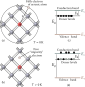
\includegraphics[scale=1]{figures/ch_05/fig_5_15.pdf}
		\caption[]{Charge carrier excitation in an n-type semiconductor: (a)---at $T=\SI{0}{\kelvin}$, the atoms of pentavalent arsenic in the germanium lattice are in a nonionized state; (b)---ionization of arsenic atoms and generation of conduction electrons at $T>\SI{0}{\kelvin}$; (c)---energy levels of one of the five electrons of every arsenic atom are donor levels; (d)---electron transition from a donor level to the conduction band at $T>\SI{0}{\kelvin}$.}
		\label{fig:5_15}
	\end{center}
	\vspace{-0.7cm}
\end{figure}

\textbf{Acceptor levels.} Let us suppose now that some of the germanium atoms in the germanium lattice are replaced by trivalent indium atoms [\fig{5_16}(a)]. The indium atom lacks one electron to establish bonds with all the four nearest neighbours. It can ``borrow'' this electron from a germanium atom. Calculations show that the necessary energy is of the order of $\ab{E}{a}\approx\SI{0.01}{\electronvolt}$. The ruptured bond corresponds to a hole [\fig{5_16}(b)] since it results in the formation of a vacant state in the valence band of germanium.

\begin{figure}[t]
	\begin{center}
		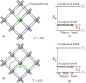
\includegraphics[scale=1]{figures/ch_05/fig_5_16.pdf}
		\caption[]{Charge carrier excitation in a p-type semiconductor: (a)---atoms of trivalent indium in the germanium lattice at $T=\SI{0}{\kelvin}$ (the fourth bond of the indium atom is unpaired); (b)---at $T>\SI{0}{\kelvin}$, the electrons can go over to unpaired bonds of impurity atoms creating an indium ion and a vacant level (hole) in the valence band of germanium; (c)---energy levels of unpaired bonds of indium atoms are acceptor levels; (d)---electron transition from the valence band to an acceptor level at $T>\SI{0}{\kelvin}$ result in the generation of holes in this band.}
		\label{fig:5_16}
	\end{center}
	\vspace{-0.7cm}
\end{figure}

Figure \ref{fig:5_16}(c) shows the band pattern of germanium doped with indium. Directly above the valence band at a distance of $\ab{E}{a}\approx\SI{0.01}{\electronvolt}$ away from it there are some empty levels of the indium atoms. Those levels are so close to the valence band that already at
relatively low temperatures, some electrons from the valence band go over to the impurity levels [\fig{5_16}(d)]. They establish bonds with the indium atoms and loose their ability to move in the germanium lattice playing no part in the conductivity. Only the holes created in the valence band act as charge carriers.

The impurities that trap electrons from the valence band are termed \textit{acceptors} and the energy levels of such impurities \textit{acceptor levels}. The semiconductors doped with such impurities are termed \textit{p-type semiconductors}.

\section{Position of the Fermi level and free carrier concentration in semiconductors}\label{sec:45}

\textbf{Dependence of free carrier concentration on the position of the Fermi level.} One of the main parameters of the gas of free carriers in a semiconductor is its chemical potential, $\mu$. As applied to the electron and hole gases the usual term for it is the \textit{Fermi level}.

As we have ascertained in Chapter \ref{chap:3}, the Fermi level in metals is the last occupied level in the conduction band (see \fig{3_4}): at absolute zero, all levels below the Fermi level are occupied by electrons and all levels above the Fermi level are empty. The concentration of the electron gas in metals is comparable, as regards its order of magnitude, to the number of states in the conduction band; because of this the gas is degenerate and the distribution of the electrons over the states is described by the Fermi-Dirac quantum statistics. The electron concentration of such a gas is practically independent of temperature.

In the intrinsic and low-doped impurity semiconductors the electron (the hole) gas is nondegenerate and the distribution of electrons over the states is described by the Maxwell-Boltzmann classical statistics. For such semiconductors the free carrier concentration is dependent on the position of the Fermi level and on temperature. Let us find this dependence.

Figure \ref{fig:5_17} shows the band pattern of a nondegenerate semiconductor. At some temperature $T$ other than absolute zero, there are some electrons in the conduction band of such a semiconductor and some holes in its valence band. Denote their concentrations by $n$ and $p$, respectively. Take as the zero energy level the bottom of the conduction band. Choose a small energy interval $\deriv{E}$ lying between $E$ and $E+\deriv{E}$ close to the bottom of the conduction band. Since the electron gas in a semiconductor is a nondegenerate gas, the number of electrons $\deriv{n}$ in the energy interval $\deriv{E}$ (per unit volume of
semiconductor) may be calculated with the aid of \eqn{3_28}:
\begin{equation}\label{eq:5_29}
    \deriv{n} = \frac{4\pi}{h^3}(2\ab{m}{n})^{3/2} e^{\mu/(\ab{k}{B}T)} e^{-E/(\ab{k}{B}T)} E^{1/2}\, \deriv{E}.
\end{equation}

\begin{figure}[t]
	\begin{center}
		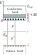
\includegraphics[scale=1]{figures/ch_05/fig_5_17.pdf}
		\caption[]{Band pattern of a nondegenerate semiconductor: $\ab{E}{c}$ is the bottom of conduction band, $\ab{E}{v}$ the top of valence band, $\mu$ the Fermi level, and $\ab{E}{g}$ the forbidden band width.}
		\label{fig:5_17}
	\end{center}
	\vspace{-0.75cm}
\end{figure}

In nondegenerate semiconductors $\mu$ is negative [see \eqn{3_48}]. This means that the Fermi level in such semiconductors is below the bottom of the conduction band, as shown in \fig{5_17}. Denote the distance from the bottom of the conduction band to the Fermi level and from the Fermi level to the top of the valence band by $\mu$ and $\mu'$, respectively. Evidently
\begin{equation}\label{eq:5_30}
    \mu+\mu' = -\ab{E}{g},\quad \text{or}\quad \mu'=-\parenthesis{\ab{E}{g}+\mu}
\end{equation}

\noindent
where $\ab{E}{g}$ is the width of the forbidden band of the semiconductor.

To obtain the total number of electrons in the conduction band at temperature $T$ we integrate \eqn{5_29} over the energy values corresponding to the conduction band, that is, from $0$ to $\ab{E}{top}$:
\begin{equation*}
    n = 4\pi \parenthesis{\frac{2\ab{m}{n}}{h^2}}^{3/2} e^{\mu/(\ab{k}{B}T)} \int_0^{\ab{E}{top}} e^{-E/(\ab{k}{B}T)} E^{1/2}\, \deriv{E}.
\end{equation*}

\noindent
The function $e^{-E/(\ab{k}{B}T)}$ decreases very rapidly as $E$ grows; therefore, it is permissible to substitute infinity for the upper limit to obtain
\begin{equation*}
    n = 4\pi \parenthesis{\frac{2\ab{m}{n}}{h^2}}^{3/2} e^{\mu/(\ab{k}{B}T)} \int_0^{\infty} e^{-E/(\ab{k}{B}T)} E^{1/2}\, \deriv{E}.
\end{equation*}

\noindent
Evaluation of this integral yields
\begin{equation}\label{eq:5_31}
    n = 2 \parenthesis{\frac{2 \pi \ab{m}{n} \ab{k}{B}T}{h^2}}^{3/2} e^{\mu/(\ab{k}{B}T)}.
\end{equation}

\noindent
A similar calculation carried out for holes generated in the valence band yields the expression
\begin{equation}\label{eq:5_32}
    p = 2 \parenthesis{\frac{2 \pi \ab{m}{p} \ab{k}{B}T}{h^2}}^{3/2} e^{-(\ab{E}{g}+\mu)/(\ab{k}{B}T)} = 2 \parenthesis{\frac{2 \pi \ab{m}{p} \ab{k}{B}T}{h^2}}^{3/2} e^{\mu'/(\ab{k}{B}T)}
\end{equation}

\noindent
where $\ab{m}{p}$ is the effective mass of the hole.

It follows from Eqs. \eqref{eq:5_31} and \eqref{eq:5_32} that the concentration of free charge carriers in a band is determined by the distance from the boundary of this band to the Fermi level: the greater this distance the smaller the carrier concentration (since $\mu<0$ and $\mu'<0$).

According to Eqs. \eqref{eq:5_31} and \eqref{eq:5_32} the product of $n$ and $p$ for any nondegenerate semiconductor is
\begin{equation}\label{eq:5_33}
    np = 4 \parenthesis{\frac{2 \pi \ab{k}{B}T}{h^2}}^3 \parenthesis{\ab{m}{n}\ab{m}{p}}^{3/2} e^{-\ab{E}{g}/(\ab{k}{B}T)}.
\end{equation}

Formula \eqref{eq:5_33} shows that for a definite temperature the product of the electron and hole concentrations is a constant for the respective semiconductor. This is an expression of the law of mass action as applied to the free carrier gas in semiconductors.

Let us now discuss separately the position of the Fermi level and the free carrier concentration in intrinsic and impurity semiconductors.

\textbf{Position of Fermi level and carrier concentration in intrinsic semiconductors.} In intrinsic semiconductors the concentration of electrons in the conduction band, $\ab{n}{i}$, is equal to that of holes in the valence band, $\ab{p}{i}$:
\begin{equation}\label{eq:5_34}
    \ab{n}{i} = \ab{p}{i}
\end{equation}

\noindent
since every electron that goes over to the conduction band leaves behind a hole in the valence band. Equating right-hand sides of Eqs. \eqref{eq:5_31} and \eqref{eq:5_32}, we obtain
\begin{equation*}
    2 \parenthesis{\frac{2 \pi \ab{m}{n} \ab{k}{B}T}{h^2}}^{3/2} e^{\mu/(\ab{k}{B}T)} = 2 \parenthesis{\frac{2 \pi \ab{m}{p} \ab{k}{B}T}{h^2}}^{3/2} e^{-(\ab{E}{g}+\mu)/(\ab{k}{B}T)}.
\end{equation*}

\noindent
Solving this equation for $\mu$, we obtain
\begin{equation}\label{eq:5_35}
    \mu = - \frac{\ab{E}{g}}{2} + \frac{3}{4} \ab{k}{B} T \ln\parenthesis{\frac{\ab{m}{p}}{\ab{m}{n}}}.
\end{equation}

This relation determines the position of the Fermi level in intrinsic semiconductors. At absolute zero ($T=\SI{0}{\kelvin}$)
\begin{equation}\label{eq:5_36}
    \mu = - \frac{\ab{E}{g}}{2}
\end{equation}

\noindent
that is, the position of the Fermi level is exactly the middle of the forbidden band (\fig{5_18}). As the temperature rises the Fermi level shifts upwards towards the bottom of the conduction band if $\ab{m}{p}>\ab{m}{n}$, and downwards towards the top of the valence band it $\ab{m}{p}<\ab{m}{n}$. In many cases, however, the shift is so small that the Fermi level in intrinsic semiconductors can be considered to be always in the middle of the forbidden band. Substituting $\mu$ from \eqn{5_35} into \eqref{eq:5_31} and \eqref{eq:5_32}, we obtain
\begin{equation}\label{eq:5_37}
    \ab{n}{i} = \ab{p}{i} = 2 \parenthesis{\frac{2 \pi \sqrt{\ab{m}{n} \ab{m}{p}} \ab{k}{B} T}{h^2}}^{3/2} e^{-\ab{E}{g}/(2\ab{k}{B}T)}.
\end{equation}

\begin{figure}[t]
	\begin{center}
		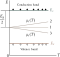
\includegraphics[scale=1]{figures/ch_05/fig_5_18.pdf}
		\caption[]{Position of Fermi level in an intrinsic semiconductor at various temperatures: at $T=\SI{0}{\kelvin}$ the Fermi level is in the middle of the forbidden band; as temperature rises the Fermi level does not change its position if $\ab{m}{n}=\ab{m}{p}$ (straight line $1$), shifts upwards if $\ab{m}{n}<\ab{m}{p}$ (straight line $2$), and shifts downwards if $\ab{m}{n}>\ab{m}{p}$ (straight line $3$).}
		\label{fig:5_18}
	\end{center}
	\vspace{-0.7cm}
\end{figure}

It follows from \eqn{5_37} that the equilibrium carrier concentration in an intrinsic semiconductor is determined by the width of the forbidden band and the temperature of the semiconductor, and the dependence on $T$ and $\ab{E}{g}$ is very strong. For instance, at room temperature a decrease in $\ab{E}{g}$ from \SI{1.12}{\electronvolt} (silicon) to \SI{0.08}{\electronvolt} (gray tin) results in an increase in nine orders of magnitude of $n$. An increase
in the temperature of germanium from \SI{100}{\kelvin} to \SI{600}{\kelvin} increases $n$ by $17$ orders of magnitude.

Using \eqn{5_37}, we may rewrite the law of mass action \eqref{eq:5_33} as
\begin{equation}\label{eq:5_38}
    np = \ab{n}{i}^2.
\end{equation}

\textbf{Position of Fermi level and carrier concentration in impurity semiconductors.} Figure \ref{fig:5_19} shows the change in the Fermi level position with the increase in temperature for (a) n- and (b) p-type semiconductors.

\begin{figure}[t]
	\begin{center}
		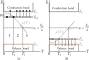
\includegraphics[scale=1]{figures/ch_05/fig_5_19.pdf}
		\caption[]{Variation of Fermi level position with temperature: (a)---in n-type semiconductors; (b)---in p-type semiconductors ($\ab{T}{s}$ is the saturation temperature of impurity levels and $\ab{T}{i}$ the temperature of transition to intrinsic conductivity).}
		\label{fig:5_19}
	\end{center}
	\vspace{-0.7cm}
\end{figure}
\begin{figure}[!h]
	\begin{minipage}[h]{0.48\linewidth}
		\begin{center}
			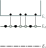
\includegraphics[scale=1]{figures/ch_05/fig_5_20.pdf}
			\caption[]{Excitation of the electrons occupying a donor level and their transition to the conduction band.}
			\label{fig:5_20}
		\end{center}
	\end{minipage}
	\hfill{ }%\hspace{-0.1cm}
	\begin{minipage}[h]{0.48\linewidth}
		\begin{center}
			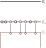
\includegraphics[scale=1]{figures/ch_05/fig_5_21.pdf}
			\caption[]{Excitation of the electrons occupying the valence band and their transition to an acceptor level.}
			\label{fig:5_21}
		\end{center}
	\end{minipage}
\vspace{-0.3cm}
\end{figure}

\textit{The low temperature range.} At low temperatures the average energy of lattice thermal vibrations, $\ab{k}{B}T$, is much less than the width of the forbidden band, $\ab{E}{g}$, and because of that, the vibrations are incapable of providing sufficient excitation of the electrons of the valence band to shift them to the conduction band. But this energy is enough to excite and shift to the conduction band the electrons occupying the donor levels $\ab{E}{d}$ (\fig{5_20}) and to the valence band the holes occupying the acceptor levels $\ab{E}{a}$ (\fig{5_21}), since this requires an energy $100$ times less than $\ab{E}{g}$. Therefore, at low temperatures practically only the ``impurity'' charge carriers—electrons in the n-type semiconductors and holes in the p-type---are excited in impurity semiconductors.

Calculations show that the position of the Fermi level inside this temperature range is
\begin{equation}\label{eq:5_39}
    \mu = -\frac{\ab{E}{d}}{2} + \frac{\ab{k}{B}T}{2} \ln\bracket{\frac{\ab{N}{d} h^3}{2 \parenthesis{2\pi \ab{m}{n} \ab{k}{B} T}^{3/2}}}
\end{equation}

\noindent
for the n-type semiconductors, and
\begin{equation}\label{eq:5_40}
    \mu' = -\frac{\ab{E}{a}}{2} + \frac{\ab{k}{B}T}{2} \ln\bracket{\frac{\ab{N}{a} h^3}{2 \parenthesis{2\pi \ab{m}{p} \ab{k}{B} T}^{3/2}}}
\end{equation}

\noindent
for the p-type semiconductors, $\ab{N}{d}$ and $\ab{N}{a}$ being the concentrations of the donors and acceptors. Graphs of the temperature dependence of $\mu$ corresponding to those functions are presented in \fig{5_19}(a, b).

Substituting $\mu$ and $\mu'$ from \eqref{eq:5_39} and \eqref{eq:5_40} into \eqref{eq:5_31} and \eqref{eq:5_32}, respectively, we obtain the following expressions for the concentrations:
\begin{equation}\label{eq:5_41}
    n = \sqrt{2\ab{N}{d}} \parenthesis{\frac{2\pi \ab{m}{n} \ab{k}{B} T}{h^2}}^{3/2} e^{-\ab{E}{d}/(2\ab{k}{B}T)}
\end{equation}

\noindent
of electrons in the n-type semiconductors and
\begin{equation}\label{eq:5_42}
    p = \sqrt{2\ab{N}{a}} \parenthesis{\frac{2\pi \ab{m}{p} \ab{k}{B} T}{h^2}}^{3/2} e^{-\ab{E}{a}/(2\ab{k}{B}T)}
\end{equation}

\noindent
of holes in the p-type semiconductors.

\textit{The impurity exhaustion range (extrinsic range).} As temperature rises, the electron concentration in the conduction band increases and that on the donor levels decreases---the donor levels become exhausted. The behaviour of acceptor levels in p-type semiconductors is similar.

In case of complete exhaustion the electron concentration in the conduction band of an n-type semiconductor becomes practically equal to the concentration of donor impurity, $\ab{N}{d}$:
\begin{equation}\label{eq:5_43}
    n \approx \ab{N}{d}
\end{equation}

\noindent
and the hole concentration in a p-type semiconductor, to that of acceptor impurity, $\ab{N}{a}$:
\begin{equation}\label{eq:5_43p}
    p \approx \ab{N}{a}.\tag{5.43$'$}
\end{equation}

\noindent
The \textit{exhaustion}, or \textit{saturation}, temperature of the impurity levels, $\ab{T}{s}$, is the higher the higher the impurity's activation energy, $\ab{E}{d}$ or $\ab{E}{a}$, and its concentration. For instance, for germanium with $\ab{N}{d}=\SI{e22}{\per\metre\cubed}$ and $\ab{E}{d}=\SI{0.01}{\electronvolt}$ the saturation temperature is approximately \SI{30}{\kelvin}.

\textit{The high temperature range.} As the temperature is raised still higher the excitation of intrinsic carriers becomes more intense, the semiconductor increasingly approaching the state of an intrinsic semiconductor with the Fermi level approaching the position of that in an intrinsic semiconductor. Until the concentration of intrinsic carriers remains much less than $\ab{N}{d}$ ($\ab{n}{i}\ll\ab{N}{d}$), the total concentration $n=\ab{n}{i}+\ab{N}{d}$ remains practically constant and equal approximately to $\ab{N}{d}$.

However, at sufficiently high temperatures the intrinsic carrier concentration may not only become equal to $\ab{N}{d}$ but may substantially exceed it ($\ab{n}{i}\gg\ab{N}{d}$). In this case $n=\ab{n}{i}+\ab{N}{d}$ is approximately $\ab{n}{i}$ and marks the transition to intrinsic conductivity. The temperature $\ab{T}{i}$ of such transition is the higher the greater is the width of the forbidden band and the impurity concentration.
For germanium with $\ab{N}{d}=\SI{e22}{\per\metre\cubed}$ this temperature is \SI{450}{\kelvin}.

Above $\ab{T}{i}$, the Fermi level in an impurity semiconductor coincides with the Fermi level in an intrinsic semiconductor and is expressed by \eqn{5_35}, its carrier concentration being identical to that of an intrinsic semiconductor at that temperature, as described by \eqn{5_37}. Figure \ref{fig:5_22} shows schematically the dependence of the natural logarithm of the electron concentration in the conduction band of an n-type semiconductor on the reciprocal temperature.
Three sections may be marked on the curve: $1$, corresponding to impurity conduction; $2$, corresponding to the impurity exhaustion range; and $3$, corresponding to intrinsic conductivity.

\begin{figure}[t]
	\begin{center}
		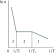
\includegraphics[scale=0.95]{figures/ch_05/fig_5_22.pdf}
		\caption[]{Temperature dependence of electron concentration in n-type semiconductors: $1$---impurity conductivity range, $2$---impurity exhaustion range, $3$---intrinsic conductivity range.}
		\label{fig:5_22}
	\end{center}
	\vspace{-0.7cm}
\end{figure}

Finally, it should be pointed out that in contrast to intrinsic semiconductors, in which both electrons and holes simultaneously take part in electrical conductivity, in impurity semiconductors the conductivity is mainly due to charge carriers of one sign: to electrons in the n-type semiconductors and to holes in the p-type. Such carriers are termed \textit{majority carriers}.

Apart from them, a semiconductor always contains minority carriers as well: n-type semiconductors contain holes and p-type semiconductors, electrons. Equilibrium carrier concentrations may be conveniently denoted as follows: $n_{n0}$ and $p_{n0}$ are the concentrations of electrons (majority carriers) and holes (minority carriers) in n-type semiconductors, $p_{p0}$ and $n_{p0}$ are the concentrations of holes (majority carriers) and electrons (minority carriers) in p-type semiconductors.

Using this notation, we may write the law of mass action \eqref{eq:5_38} in the following form:
\begin{equation}\label{eq:5_44}
    n_{n0} p_{n0} = \ab{n}{i}^2,\quad p_{p0} n_{p0} = n^2.
\end{equation}

\noindent
It follows from \eqn{5_44} that doping a semiconductor by an electrically active impurity, while increasing the majority carrier concentration, should inevitably decrease the minority carrier concentration so as to keep the product of those concentrations constant.

\section{Nonequilibrium carriers}\label{sec:46}

As we already know, at all temperatures other than absolute zero a process of \textit{free carrier excitation}, or \textit{generation}, takes place in the semiconductor. Should this be the only process taking place, the carrier concentration would continuously grow with time. However, there is a simultaneous process of \textit{free carrier recombination}. The essence of this process is that when a free electron meets a hole it may occupy it, the result being annihilation of a pair of carriers.

At any temperature, an equilibrium is established between the processes of thermal carrier generation and recombination characterized by appropriate equilibrium carrier concentrations. Such carriers are termed \textit{equilibrium carriers}. The law of mass action discussed in the previous section is applicable only to them.

Besides thermal excitation, there are other methods of free carrier generation in semiconductors: by light, by ionizing particles, by injection through a contact, and others. Such factors result in the appearance of additional free carriers, \textit{excess carriers}, as compared with the equilibrium carrier concentration. Another term for them is \textit{nonequilibrium carriers}. Denote the concentrations of such carriers by $\Delta{n}$ and $\Delta{p}$, respectively. Then the total carrier concentration will be
\begin{equation}\label{eq:5_45}
    n = n_0 + \Delta{n},\quad p = p_0 + \Delta{p}
\end{equation}

\noindent
where $n_0$ and $p_0$ are the equilibrium carrier concentrations.

Every nonequilibrium carrier having been born in the semiconductor ``lives'' a limited time before recombining, the time being different for different carriers. For this reason, an average carrier lifetime $\tau$ is introduced, with the notation $\ab{\tau}{n}$ for electrons and $\ab{\tau}{p}$ for holes.

The carrier generation process is characterized by the \textit{generation rate} $g$, which expresses the number of carriers (or carrier pairs) generated in a unit volume of the semiconductor per second.

The recombination process is characterized by the \textit{recombination rate} $R$, which is equal to the number of carriers (carrier pairs) recombining in a unit volume of the semiconductor per second. For electrons
\begin{equation}\label{eq:5_46}
    \ab{R}{n} = -\diff{n}{t} = - \diff{(\Delta{n})}{t}
\end{equation}

\noindent
and for holes
\begin{equation}\label{eq:5_47}
    \ab{R}{p} = -\diff{p}{t} = - \diff{(\Delta{p})}{t}
\end{equation}

\noindent
where $n$ and $p$ are the total concentrations of electrons and holes, respectively, at a given moment of time; $\Delta{n}$ and $\Delta{p}$ are the respective
excess concentrations at the same moment; and the minus signs point to the fact that recombination results in a decrease in carrier concentrations.

Suppose that light generates excess carriers in a semiconductor whose concentrations are $\Delta{n}_0=\Delta{p}_0$. After the light is turned off, those carriers will recombine and their concentrations shall gradually diminish. Since every excess carrier, for instance, an electron, lives on the average $\ab{\tau}{n}$, their recombination rate will be $\Delta{n}/\tau$ per second, where $\Delta{n}$ is the excess carrier concentration at the moment. Therefore, the recombination rate is
\begin{equation}\label{eq:5_48}
    \ab{R}{n} = - \diff{(\Delta{n})}{t} = \frac{\Delta{n}}{\ab{\tau}{n}}.
\end{equation}

\noindent
A similar relation holds for holes:
\begin{equation}\label{eq:5_49}
    \ab{R}{p} = - \diff{(\Delta{p})}{t} = \frac{\Delta{p}}{\ab{\tau}{p}}.
\end{equation}

\noindent
Integrating the two equations, we obtain
\begin{equation}\label{eq:5_50}
    \Delta{n} = \Delta{n}_0\, e^{-t/\ab{\tau}{n}},\quad \Delta{p} = \Delta{p}_0\, e^{-t/\ab{\tau}{p}}.
\end{equation}

\noindent
It follows from \eqn{5_50} that $\Delta{n}=\Delta{n}_0/e$ and $\Delta{p}=\Delta{p}_0/e$ for $t=\tau$. Hence, the average excess carrier lifetime is a time interval during which the carrier concentration due to recombination decreases $e=2.73$ times.

Free charge carriers diffuse in the volume of the semiconductor and during their lifetime $\tau$ cover an average distance $L$ termed \textit{carrier diffusion length}. Calculations show that $L$ depends on $\tau$ in the following manner:
\begin{equation}\label{eq:5_51}
    L = \sqrt{D t}
\end{equation}

\noindent
where $D$ is the \textit{carrier diffusion coefficient}, related to their mobility $u$ by the Einstein relation
\begin{equation}\label{eq:5_52}
    D = \frac{\ab{k}{B} T u}{q}
\end{equation}

\noindent
where $q$ is the electron charge.

The transition of the electron from the conduction to the valence band may take place directly across the whole forbidden band $\ab{E}{g}$, as shown by arrow $1$ in \fig{5_23}, or indirectly, first to the impurity level $\ab{E}{im}$ (arrow $2$) and then from this level to the valence band (arrow $3$). Recombination of the first type is termed \textit{direct recombination} and of the second type \textit{recombination via an impurity level}.

\begin{figure}[t]
	\begin{center}
		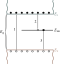
\includegraphics[scale=1]{figures/ch_05/fig_5_23.pdf}
		\caption[]{Excess charge carrier recombination in semiconductors: $1$---direct recombination, $2$ and $3$---recombination via impurity level.}
		\label{fig:5_23}
	\end{center}
	\vspace{-0.7cm}
\end{figure}

In both types of recombination the same energy $\ab{E}{g}$ is liberated. The only difference is that in the first case this energy is liberated in one act and in the second in two acts corresponding to the transitions $2$ and $3$.

The energy may be liberated in the form of a light quantum $h\nu$ or in the form of heat (phonons). In the first instance the recombination is termed \textit{radiative} and in the second \textit{nonradiative}. Calculation and experiment show that direct recombination plays an essential part in
semiconductors with a narrow forbidden band at relatively high temperatures (room temperature and above). The principal recombination mechanism in wide forbidden band semiconductors is nonradiative recombination via impurity, or defect, levels. However, under appropriate conditions a relatively high level of radiative recombination may be attained even in such semiconductors. A favourable factor is, for instance, the increase in excess carrier concentration and in some cases higher doping. A remarkable material in this respect is gallium arsenide (\ce{GaAs}) in which, given favourable conditions, radiative recombination may constitute as high as $50\%$ or higher of the total. For this reason, gallium arsenide is at present the principal material for making luminescent diodes and
semiconductor lasers, which find wide practical use.
